\subsection*{Partie A}
\begin{enumerate}
	\item L'arbre de probabilité représentant la situation est :

	
	\begin{center}
		
		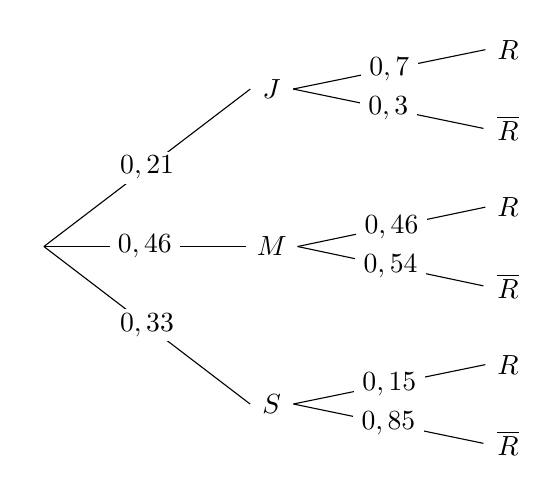
\begin{tikzpicture}[xscale=1,yscale=1]
			
			\tikzstyle{noeud}=[fill=white,circle,inner sep=2pt]
			\tikzstyle{feuille}=[fill=white,circle,inner sep=2pt]
			\tikzstyle{etiquette}=[midway,fill=white, inner xsep=3pt, inner ysep=1.5pt]
			
			\def\DistanceInterNiveaux{3}
			\def\DistanceInterFeuilles{1}
			
			\def\NiveauA{(0)*\DistanceInterNiveaux}
			\def\NiveauB{(1)*\DistanceInterNiveaux}
			\def\NiveauC{(2)*\DistanceInterNiveaux}
			\def\InterFeuilles{(-1)*\DistanceInterFeuilles}
			
			\node[noeud] (R) at ({\NiveauA},{(2.5)*\InterFeuilles}) {};
			\node[noeud] (Ra) at ({\NiveauB},{(0.5)*\InterFeuilles}) {$J$};
			\node[feuille] (Raa) at ({\NiveauC},{(0)*\InterFeuilles}) {$R$};
			\node[feuille] (Rab) at ({\NiveauC},{(1)*\InterFeuilles}) {$\overline{R}$};
			\node[noeud] (Rb) at ({\NiveauB},{(2.5)*\InterFeuilles}) {$M$};
			\node[feuille] (Rba) at ({\NiveauC},{(2)*\InterFeuilles}) {$R$};
			\node[feuille] (Rbb) at ({\NiveauC},{(3)*\InterFeuilles}) {$\overline{R}$};
			\node[noeud] (Rc) at ({\NiveauB},{(4.5)*\InterFeuilles}) {$S$};
			\node[feuille] (Rca) at ({\NiveauC},{(4)*\InterFeuilles}) {$R$};
			\node[feuille] (Rcb) at ({\NiveauC},{(5)*\InterFeuilles}) {$\overline{R}$};
			
			\draw (R.east)--(Ra.west) node[etiquette]{$0,21$};
			\draw (Ra.east)--(Raa.west) node[etiquette]{$0,7$};
			\draw (Ra.east)--(Rab.west) node[etiquette]{$0,3$};
			\draw (R.east)--(Rb.west) node[etiquette]{$0,46$};
			\draw (Rb.east)--(Rba.west)  node[etiquette]{$0,46$};
			\draw (Rb.east)--(Rbb.west)  node[etiquette]{$0,54$};
			\draw (R.east)--(Rc.west)  node[etiquette]{$0,33$};
			\draw (Rc.east)--(Rca.west)  node[etiquette]{$0,15$};
			\draw (Rc.east)--(Rcb.west)  node[etiquette]{$0,85$};
		\end{tikzpicture}
	\end{center}
	


	\item  $P(M \cap R)= P(M) \times P_M(R)= 0,46 \times 0,46 = 0,2116$.

	La probabilité que la personne interrogée ait entre 30 et 59 ans et ait déjà publié sur ce réseau social est égale à 0,2116 (valeur exacte).



	\item

	\begin{enumerate}
		\item Calculons la probabilité qu'une personne ait déjà publié sur ce réseau social, c'est à dire calculons $P(R)$.

		Les événements $J$, $M$ et $S$ forment une partition de l'univers, donc, d'après la loi des probabilités totales on a :

		$\begin{aligned}
			P(R) & = P(J \cap R) + P(M \cap R) + P(S \cap R) \\
			&= P(J) \times P_J(R) + P(M) \times P_M(R) + P(S) \times P_S(R) \\
			&= 0,21 \times 0,7 + 0,46 \times 0,46 + 0,33 \times 0,15 \\
			&= 0,4081
		\end{aligned}$

		La probabilité que la personne ait déjà publié sur ce réseau social est égale à 0,4081 (valeur exacte).

		\item Déterminons la probabilité qu'une personne ait au moins 60 ans sachant qu'elle a déjà publié sur ce réseau social, c'est à dire calculons $P_R(S)$

		$P_R(S)= \dfrac{P(R\cap S)}{P(R)}= \dfrac{0,33 \times 0,15}{0,4081} \approx 0,12129$

		La probabilité qu'une personne ait au moins 60 ans sachant qu'elle a déjà publié sur ce réseau social est égale à 0,121 arrondi au millième.
	\end{enumerate}
\end{enumerate}

\subsection*{Partie B}


\begin{enumerate}
	\item On admet que la variable aléatoire $X$ suit une loi binomiale, ses  paramètres sont $n=100$ et  $p=0,41$.

	\emph{Remarque :} ici, on a une rédaction plus légère, car l'énoncé demande d'admettre que $X$ suit une loi binomiale. Sinon, il faudrait les trois arguments classiques :

	\begin{itemize}
		\item On a une épreuve à deux issues, succès de probabilité $p = 0,41$ et échec;
		\item cette épreuve est répétée $n = 100$ fois, de façon identique et indépendante (car la constitution de l'échantillon est assimilé à un tirage au sort \textbf{avec} remise);
		\item $X$ est la variable aléatoire qui compte le nombre de succès sur ces $n$ répétitions.
	\end{itemize}

	\item À l'aide de la calculatrice: $P(X \geq 50) \approx 0,04279 $

	La probabilité qu'au moins la moitié des 100 personnes interrogées ait déjà publié sur ce réseau social est égale à   0,043 au millième près.

	\item  $E(X) = n\times p = 100 \times 0,41 =41$

	L'espérance de la variable aléatoire $X$ est égale à 41.

	Si on répète l'expérience un très grand nombre de fois, en moyenne 41 personnes sur les 100 auront déjà publié sur ce réseau social.
\end{enumerate}

\subsection*{Partie C}


La variable aléatoire $Y$ est définie par :
$Y=\dfrac{X_{1}+X_{2}+\cdots+X_{150}}{150}$ est la variable aléatoire  moyenne d'un échantillon  de taille 150 de la variable aléatoire $X$ on a donc :



$E\left(Y\right) = E(X)= 41$

et   $\begin{aligned}[t] V\left(Y\right) &= \dfrac{1}{150} V(X)\\
	&  =  \dfrac{100 \times 0,41 \times (1-0,41)}{150} \text{ car } X \text{ suit une loi binomiale de paramètres 100 et 0,41}\\
	&= \dfrac{24,19}{150}
\end{aligned} $


On a  : $P(37<Y<45) = P(-4< Y-41<4) = 1- P\Big(\big|Y-41\big| \geq 4\Big)$

Or, d'après l'inégalité de Bienaymé-Tchebychev :

$\forall t \in \R^{*+}, \quad P\Big(\big|Y - E(Y)\big| \geq t\Big) \leq  \dfrac{V(Y)}{t^2 } $.

Avec $t= 4$  on  a : $P\Big(\big|Y- 41\big| \geq 4\Big) \leq  \dfrac{24,19}{150 \times 4^2 } $

soit  $ P\Big(\big|Y-41\big| \geq 4\Big) \leq \dfrac{ 803}{80000}$

On a donc :  $1- P\Big(\big|Y-41\big| \geq 4\Big) \geq 1- \dfrac{ 803}{80000}$

D'où : $P(37<Y<45) \geq 0,98996$


La probabilité que la variable aléatoire $Y$ soit strictement comprise entre 37 et 45 est donc strictement supérieure à $98~\%$.
